
\chapter{Primitive Data Types}

\section{Boolean}
\iffalse
https://oopscenities.net/2011/09/28/c-primitive-types/
https://en.wikipedia.org/wiki/Primitive_data_type
http://rypress.com/tutorials/objective-c/data-types/primitives
https://en.wikipedia.org/wiki/C_data_types
\fi
\section{Character}

\section{Floating-point}

\section{Integer}

\section{Enumeration}


\chapter{Composite Data Types}
\section{Record - struct or class}
\section{Union}
\section{Tagged Union}


\chapter{Array}
Array belongs to the so called \textit{Contiguous} Data Structure in which stored elements (all of the same type) are arranged in a \textbf{single} slab of memory. Array's elements can be easily  accessed given their \textit{indices} within the array itself the same way, using an analogy, we can locate an house in a specific street given its postcode. Array can also be tought as a collection of variables of the same type.

Major characteristic of arrays are:
\begin{description}
\item [Constant time access] All the element of the array can be accessed in $\mathcal{O}(1)$. Array can be fully described by its
	\begin{enumerate}
		\item Starting address $m_0$
		\item Size of Stored data type (e.g. 4 bytes for \texttt{int} or 1 byte for \texttt{char}) $S$
		\item Number of stored elements (i.e. array length) $L$
	\end{enumerate}
	\begin{figure}[h]
		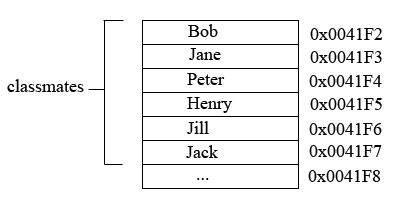
\includegraphics[width=8cm]{array1.png}
	\end{figure}
	The starting address correnspond to the first element (in C-like languages index $0$) element.
	 The second element starts at the address  $m_0 + S$, third at $m_0 + S + S$ and so on. so the element at index $i$ has index $s_i = m_0 +iS$.
	
\item [Only Data] Array are space efficient because they do not store any other information but data itself (unlike list for instance where each node of the list stores a pointer to the next element of the list). 
 
\item [Memory locality] Array adhere perfectly to the principle of spatial locality\footnote{If a particular memory location is referenced at a particular time, then it is likely that nearby memory locations will be referenced in the near future. In this case it is common to attempt to guess the size and shape of the area around the current reference for which it is worthwhile to prepare faster access.} in which related storage locations are frequently accessed (iterating through an array is a very common idiom in all programming languages). This allows cache to work at his best.
\end{description}

Arrays have fixed size, and this in several application is a major downside (the size of the array is input dependent for instance). C-like languages allow for dynamic memory allocation at runtime (see \ref{chap:malloc} at page (\pageref{{chap;malloc}}). This involves the creation of a (different) larger (how larger is an important point) array and the copy of the first one in the beginning of the newly created one. If the program requires this dynamic enlarging often we could end up wasting much time in copying data here and there.
The common strategy used for creating a dynamic array is to double the size of the array each time. This mitigate the average number of copies of each element. Let's imagine we start with an array of size one and we try to insert $n$ elements, doubling the size of the array when its capacity its full. The first element is has to be copied when the array expands after the fist, second, fourth, eighth ... $2^i = n$ insertion.
It will take $i = log(n)$ doubling size for the array to have size $n$. Element in the last half of the array will be copied only one (at the last doubling). A quarter of the elements will be copied twic and so on. The total number of copies will be then
\[
M = \sum_{i=1}^{\log(n)} \frac{ni}{2^i} = n\sum_{i=1}^{\log(n)} \frac{i}{2^i} = n(\frac{1}{2}+\frac{1}{2} + \frac{3}{8} + \frac{1}{3} ... \frac{log(n)}{n})=2n
\]
So in average  each element is copied only two times.

 \section{Problems and Solution}

%---Problem---------------------------------
\begin{problem}
Given an array, $A$, of $N$ integers, print each element in reverse order as a single line of space-separated integers.
\end{problem}	

\begin{solution}

		\begin{lstlisting}[language=C, caption="C"]
        int main(){
    int n; 
    scanf("%d",&n);
    int *arr = malloc(sizeof(int) * n);
    for(int arr_i = 0; arr_i < n; arr_i++){
       scanf("%d",&arr[arr_i]);
    }
    while(--n >=0){
       printf("%i ",arr[n]);
    }
    
    return 0;
}

		\end{lstlisting}  

\end{solution}	
%------------------------------------------------ 
 
  \begin{problem}
	Reverse an array in place.
 \end{problem}
 
 \begin{problem}
    Implement a function to determine if a string has all unique characters. String can only contains latin 	characters. What happen if you are forced to use no additional data structures?
\end{problem}

 \begin{problem}
    Implement a function to determine if a string has all unique characters. String can only contains latin 	characters. What happen if you are forced to use no additional data structures?
\end{problem}

 \begin{problem}
    Implement a function to determine the number of repeated characters in a string. (e.g. google has 2 repeated characters, \textit{g} and \textit{o}).
\end{problem}

 \begin{problem}
   Given an array of integer of given size containing numbers from 1 to $N \geq 2$ . Only one number is missing within the array. Write a function which output is that missing number.
\end{problem}

 \begin{problem}
   Given an array of integer of size $N$ containing numbers from 1 to $N-2$. All numbers appear only once except one which is repeated twice. Write a function which return that number.
\end{problem}

 \begin{problem}
Write a function which find the smallest and largest number in an unsorted array of integers. 
\end{problem}

 \begin{problem}
	Sort an array of integer using a $\mathcal{O}(n^2)$  and a $\mathcal{O}(nlog(n))$  algorithm. Both algorithm should sort the array \textit{in-place}.
\end{problem}

 \begin{problem}
	Given two array of sorted integer, \textit{A,B} find their intersection i.e. an array $C$ which contains only elements which belong both to A and B. $C=\{c_i \;|\; c_i \in A;,\; c_i \in B\}$
\end{problem}

 \begin{problem}
	Given two array of unsorted integer in which only one element is repeted (the rest of them appear only once). Write a function which finds that element in $\mathcal{O}(n)$  time.
\end{problem}

 \begin{problem}
	Write a function which finds the kth largest element in a unsorted array.
\end{problem}
 \begin{problem}
	Write a function which finds the kth smallest element in a unsorted array.
\end{problem}

 \begin{problem}
Count the number of distinct ( (a,b) is not distinct from (b,a) ) pairs in an array of integers which sum is equal to a given value $K$.
\end{problem}

 \begin{problem}
Given three sorted array (in non decreasing order) find the intersection between all of their elements.
\end{problem}

 \begin{problem}
Given an array, find the first repeated element. i.e. an element $e$ which occurs more than once and which index is the smallest. On the following input $1,2,3,4,5,3,2,2,7$ the function should return two because is the a repeated element with the smallest index (1).
\end{problem}

 \begin{problem}
Given an array, return the larger and the 2th-largst element.
\end{problem}


 \begin{problem}
Given an array of integer, find the smallest positive integer which cannot be represented as sum of any subset of the array. On  input 1, 3, 6, 10, 11, 15 the function should return 2. Note that the array can also contains negative numbers.
\end{problem}

 \begin{problem}
Given an array of integer (positive and negative), return an array which elements are rearranged in alternating positive and negative. You are ensured that the number of positives and negatives matches. E.g. on input $(1,2,-6,4,8,-6,-5)$ the functions (only one of the possible valide output) return $(1,-6,2,-6,4,-5,8)$.
\end{problem}

 \begin{problem}
Given an array of integer write a function which return true is a non empty subset of its element which sum up to $0$. False otherwise. 
\end{problem}

 \begin{problem}
Given an array $A$ of integer find the length of the  longest sequence of consecutive integers. On input $1,56,8,-5,3,7,4,23,2,5)$ the function should return 5 (is the length of the consecutive subsequence $(1,2,3,4,5)$)
 \end{problem}

 \begin{problem}
Find the minimum in a rotated sorted array. (a rotation of $1,2,3,4,5,6$ could be for instance $4,5,6,1,2,3$). The array does not contains duplicates.

What if we allows for duplicated to be present? How does this changes the overall time complexity?
 \end{problem}

 \begin{problem}\label{array:anagram}
Given two string, determine which is the minimum number of deletions (a delete operation can be performed on both string) necessary for the two string to be a valid anagram\footnote{A word, phrase, or name formed by rearranging the letters of another, such as spar, formed from rasp.} of each other. Strings contains only latin characters with no space. Given \textit{hello} and \textit{belloz} the function should returns 2. ( See solution \ref{array:anagram_sol} at page \pageref{array:anagram_sol} )


\begin{lstlisting}[ label=array:anagram_sol, caption=Solution to problem \ref{array:anagram} ]
#include <stdio.h>
#include <string.h>
#include <math.h>
#include <stdlib.h>

void removeTrailingNL(char* s){
    int size = strlen(s);
    if(size > 0 && s[size-1] == '\n')
        s[size-1] = '\0';
}

#define MAX_INPUT_SIZE (10000)
int main() {
    const int alph_size = 'z'-'a'+1;
    int s1_freq[alph_size];
    int s2_freq[alph_size];
    //initialize frequencies arrays
    for(int i = 0 ; i < alph_size ; i++){
        s1_freq[i] = 0;
        s2_freq[i] = 0;
    }
    //read both string
    char s1[10000];
    char s2[10000];
    fgets(s1,MAX_INPUT_SIZE,stdin);
    fgets(s2,MAX_INPUT_SIZE,stdin);
    removeTrailingNL(s1);
    removeTrailingNL(s2);
    
    int size_s1, size_s2;
    size_s1 = strlen(s1);
    size_s2 = strlen(s2);
    //compute frequencies
    for(int i  = 0 ; i< size_s1 ; i++)
        s1_freq[s1[i]-'a'] = s1_freq[s1[i]-'a'] + 1;
    for(int i  = 0 ; i< size_s2 ; i++)
        s2_freq[s2[i]-'a'] = s2_freq[s2[i]-'a'] + 1;
    /*
  //print frequencies  
 for(int i  = 0 ; i< alph_size ; i++){
     printf("%c %i %i\n",'a'+i,s1_freq[i],s2_freq[i]);
 }*/
    
    //compute minimum delete operation
    int dels = 0;
    for(int i  = 0 ; i< alph_size ; i++)
        dels = dels + (abs(s1_freq[i] - s2_freq[i]));
    
    
    //prints output
    printf("%i",dels);
   
    return 0;
}
\end{lstlisting}
 \end{problem}






\chapter{List}
\section{Singly Linked List}
\section{Doubly Linked List}
\section{Circular Linked List}
\section{Self-Organizing Lists}
\section{Skip Lists}

\chapter{Stack}

\chapter{Queue}
\section{Double-ended queue - Dequeue}

\section{Priority Queue}
Nevertheless, the heap data structure itself has enormous utility. In this section, we present one of the most popular applications of a heap: its use as an efficient priority queue.
A priority queue is a data structure for maintaining a set S of elements, each with an associated value called a key. A priority queue supports the following operations.
\begin{description}
\item [\texttt{INSERT(S,x)}] inserts an element $x$ into the set S
\item [\texttt{\{MAX,MIN\}(S,x)}] return the element of S with largest/smallest key 
\item [\texttt{EXTRACT-\{MAX,MIN\}(S,x)}] return and removes the element of S with largest/smallest key 
\end{description}
One application of priority queues is to schedule jobs on a shared computer. The priority queue keeps track of the jobs to be performed and their relative priorities. When a job is finished or interrupted, the highest-priority job is selected from those pending using EXTRACT-MAX. A new job can be added to the queue at any time using INSERT.

A priority queue can also be used in an event-driven simulator. The items in the queue are events to be simulated, each with an associated time of occurrence that serves as its key. The events must be simulated in order of their time of occurrence, because the simulation of an event can cause other events to be simulated in the future. For this application, it is natural to reverse the linear order of the priority queue and support the operations MINIMUM and EXTRACT-MIN instead of MAXIMUM and EXTRACT-MAX. The simulation program uses EXTRACT-MIN at each step to choose the next event to simulate. As new events are produced, they are inserted into the priority queue using INSERT.

Not surprisingly, we can use a heap to implement a priority queue. The operation HEAP-MAXIMUM returns the maximum heap element in (1) time by simply returning the value A[1] in the heap. The HEAP-EXTRACT-MAX procedure is similar to the for loop body (lines 3-5) of the HEAPSORT procedure:

\begin{algorithm}[H]
 \KwData{Heap H}
 \KwResult{Extract Max - Max element of H}
\uIf{heap-size(H) $<$ 1}{
	 underflow error
   }

$max \gets H[1]$\;
$H[1] \gets H[heap-size(H)]$\;
$heap-size(H) \gets heap-size(H) -1$\;
\Return{max}\;

\caption{Priority Queue Extract-max pseudocode}
\end{algorithm}

The running time of HEAP-EXTRACT-MAX is $\mathcal{O}(log n)$, since it performs only a constant amount of work on top of the $\mathcal{O}(log n)$ time for HEAPIFY.

The HEAP-INSERT procedure inserts a node into heap A. To do so, it first expands the heap by adding a new leaf to the tree. Then, in a manner reminiscent of the insertion loop of INSERTION-SORT (see section \ref{sec:insertionsort} at page \pageref{sec:insertionsort}), it traverses a path from this leaf toward the root to find a proper place for the new element.

\begin{algorithm}[H]
 \KwData{Heap H, Key key}
 \KwResult{Insert an element in the Heap H}
	$heap-size(H) \gets heap-size(H)+1$\;
	$i \gets heap-size(H)$\;
	\While{$i > 1 and H[parent(i)] < key$}{
		$H[i] \gets H[parent(i)]$\;
		$i \gets parent(i)$\;
	}
	$H[i] \gets key$
\caption{Priority Queue insert pseudocode}
\end{algorithm}

\begin{problem}
Show how to implement a first-in, first-out queue with a priority queue. Show how to implement a stack with a priority queue.
\end{problem}


\begin{problem}

Give an O(lg n)-time implementation of the procedure HEAP-INCREASE-KEY(A, i, k), which sets A[i]  max(A[i],k) and updates the heap structure appropriately.
\end{problem}

\begin{problem}

The operation HEAP-DELETE(A, i) deletes the item in node i from heap A. Give an implementation of HEAP-DELETE that runs in O(lg n) time for an n-element heap.
\end{problem}

\begin{problem}

Give an O(n lg k)-time algorithm to merge k sorted lists into one sorted list, where n is the total number of elements in all the input lists. (Hint: Use a heap for k-way merging.)
\end{problem}


\begin{problem}

A d-ary heap is like a binary heap, but instead of 2 children, nodes have d children.
\begin{enumerate}
\item How would you represent a d-ary heap in an array?
\item What is the height of a d-ary heap of n elements in terms of n and d?
\item Give an efficient implementation of EXTRACT-MAX. Analyze its running time in terms of d and n.
\item Give an efficient implementation of INSERT. Analyze its running time in terms of d and n.
\item Give an efficient implementation of HEAP-INCREASE-KEY(A, i, k), which sets A[i]  max(A[i], k) and updates the heap structure appropriately. Analyze its running time in terms of d and n.
\end{enumerate}
\end{problem}








\chapter{Heap}


\chapter{Tree}

\section{Binary Tree}
\section{Binary Search Tree}

\section{Self Balancing Tree}
\subsection{B Tree}
\subsection{B+ Tree}

\subsection{Adelson-Velsky Landis Tree - AVL Tree}
\subsection{Red Black Tree}
\subsection{Splay Tree}


\section{Space-partitioning trees}
\subsection{Kd Tree}
\subsection{R Tree}

\chapter{Graph}

\chapter{Set}
\section{MultiSet}

\chapter{Associative Array - Dictionary}
\section{Map}
\section{MultiMap}
\section{Hash table - Hash Map}
\iffalse
http://www.tommyds.it/doc/benchmark.html
\fi